\subsection{Design}
This section describes the main aspects of the VFS Browser applicatoin. It shows
the implementation of the core interfaces and classes.

\subsubsection{GUI classes}\label{sec:guiClasses}
Figure \ref{fig:gui_classes} gives an overview of the main interfaces and
classes that were implemented for the gui. The implementation followed the rules
of a MVC design dividing the aspects of Model View and Control to their
respective classes. According to the partition of MVC the classes were
partitioned into the packages \textit{model, view and controller}.

\begin{figure}[h!]
\centering
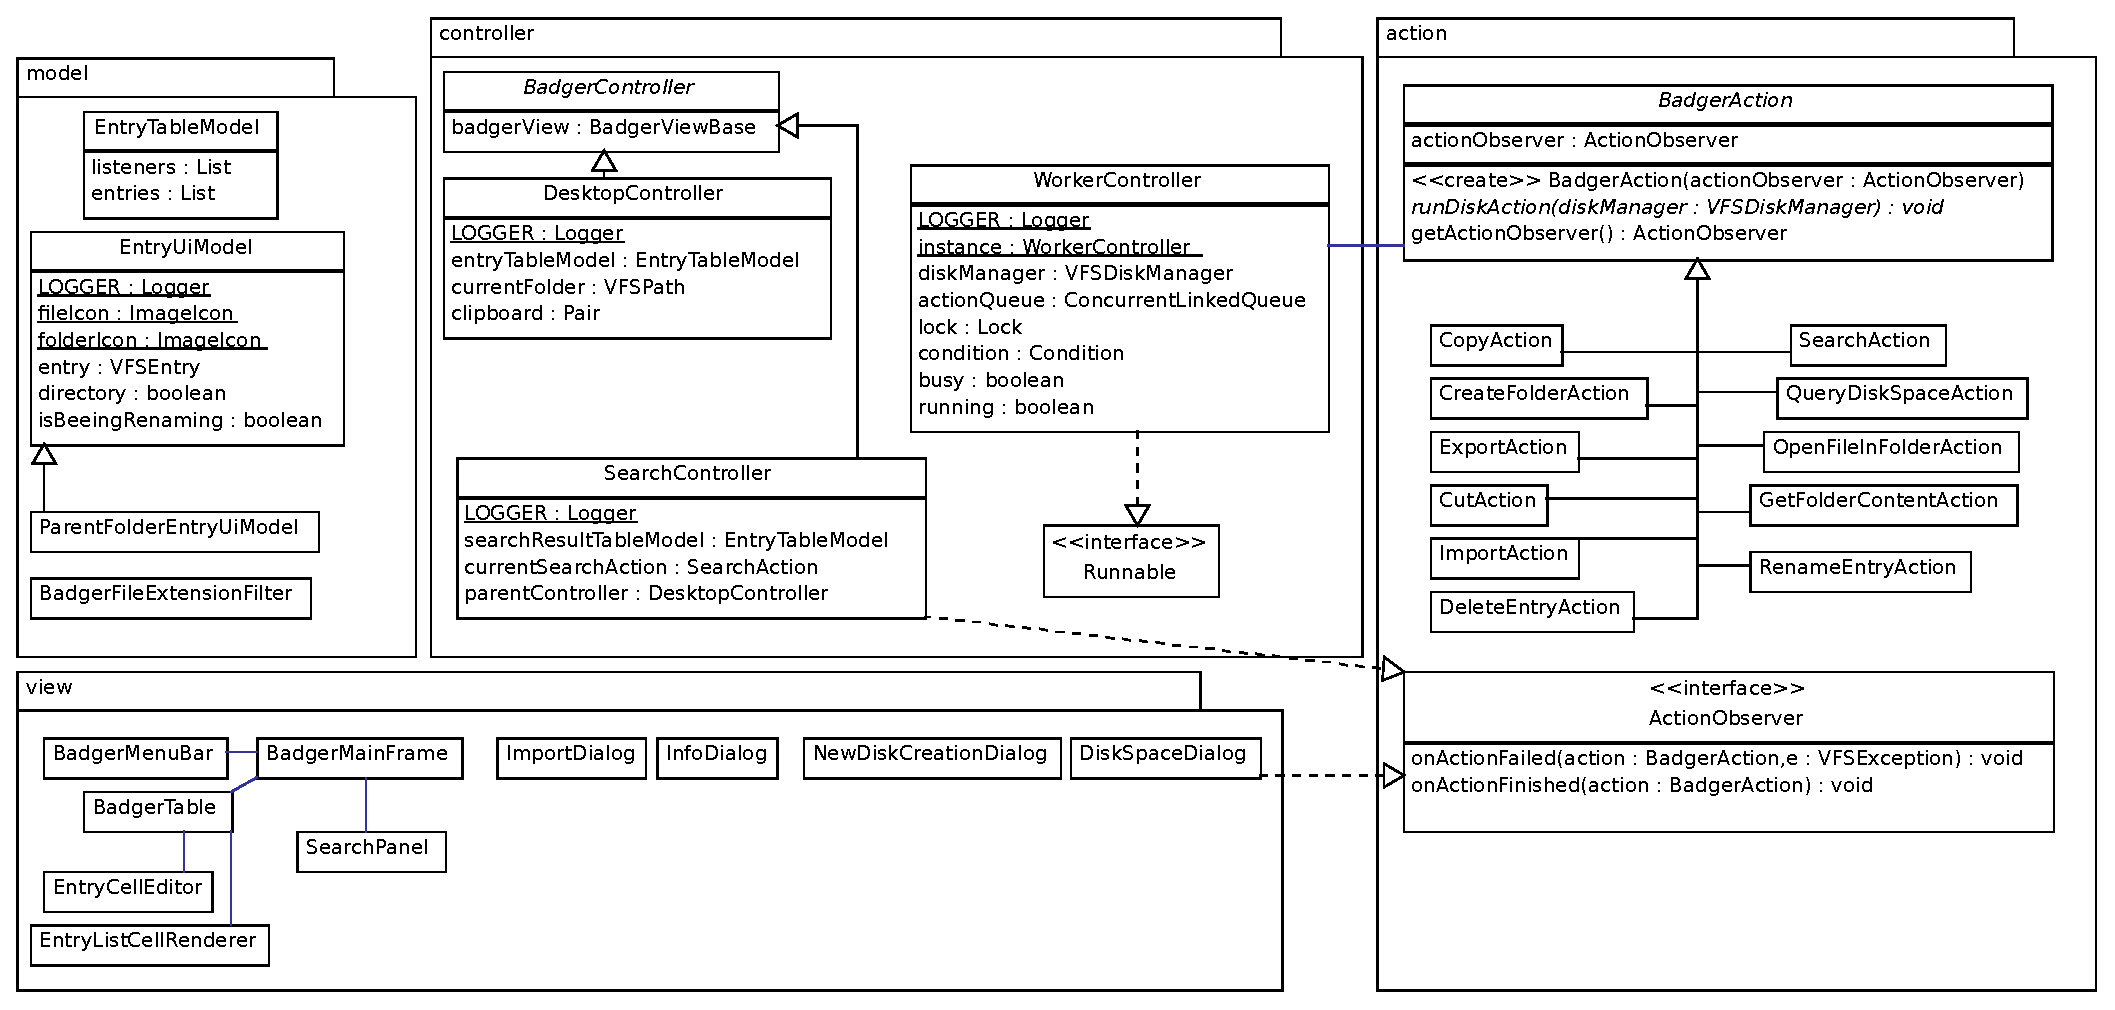
\includegraphics[width=1\textwidth]{figures/gui_classes.eps}
\caption{gui classes}
\label{fig:gui_classes}
\end{figure}


\subsubsection{Decoupling of gui and working threads}
This section describs the way how the decoupling from gui and working threads
was implemented. This decoupling mades the gui still responsive event tough some
long running tasks like importing or search would be running.


\subsubsection{Search}


\subsubsection{Keyboard and Mouse support}